%
% main.tex -- Paper zum Thema <wirbelringe>
%
% (c) 2020 Autor, OST Ostschweizer Fachhochschule
%
% !TEX root = ../../buch.tex
% !TEX encoding = UTF-8
% LTeX: enabled=false
\chapter{Wirbelringe\label{chapter:wirbelringe}}
\kopflinks{Wirbelringe}
\begin{refsection}
\chapterauthor{Nino Briker und Fabian Steiner}
\index{Nino Briker}%
\index{Briker, Nino}%
\index{Fabian Steiner}%
\index{Steiner, Fabian}%

%
% intro.tex -- Einleitung zum Thema
%
% !TEX root = ../../buch.tex
% !TEX encoding = UTF-8
%
\section{Einleitung}

Wirbelringe sind ein interessantes Naturphänomen welchem man schneller begegnet als man denkt. 
In diesem Paper schauen wir uns Wirbelringe etwas genauer an und begründen einige Eigenschaften. 
Des Weiteren untersuchen wir eine weitverbreitete praktische (ungewollte) Anwendung und dessen Auswirkung. 
Zuletzt formulieren wir ein Modell womit man zumindest angenähert selbst gezielt Wirbelringe berechnen und erzeugen kann.

In diesem Paper werden, wo nicht anders angegeben, nur ideale Fluide betrachtet.

\begin{quote}
    The theory of inviscid fluids is the study of «dry water».

    - John von Neumann \cite{Wirbelringe:feynman1964lectures}
\end{quote}

\subsection{Wirbel}

\begin{figure}
\centering
\begin{tikzpicture}
\clip (-6.3,-2.7) rectangle (6.3,2.7);
\node at (-0.07,-0.07) {\includegraphics[width=1.08\textwidth]{papers/wirbelringe/fig/flacher_wirbel.pdf}};
%\draw[color=red] (-6.3,-2.7) rectangle (6.3,2.7);
\end{tikzpicture}
\caption{Darstellung eines 2-dimensionalen Wirbels mit Wirbelvektor
\(\vec{\omega}\).
\label{Wirbelringe:fig:flacher_wirbel}}
\end{figure}


Für die Betrachtung von Wirbelringen starten wir zunächst mit einzelnen Wirbeln.
Ein Wirbel ist eine Formation von Teilchen, welche um einen Mittelpunkt rotieren.
In Abbildung \ref{Wirbelringe:fig:flacher_wirbel} ist ein Wirbel abgebildet.
Die eingezeichneten Pfeile stellen die Geschwindigkeitsvektoren \( \vec{v} \) von den Teilchen dar, welche Teil des Wirbels sind.
Nicht explizit eingezeichnet sind die Bahnen, auf welchen sich die Teilchen bewegen.
Die Bahnen bilden konzentrische Kreise.
Auch ist in der Abbildung \ref{Wirbelringe:fig:flacher_wirbel} der Wirbelstärkevektor \(\vec{\omega}\) eingezeichnet.
Wir kommen später genauer auf \(\vec{\omega}\) zu sprechen.

\subsubsection*{Wirbellinien \label{Wirbelringe:Wirbellinien}}

Um Wirbel besser zu beschreiben, führen wir hier den Begriff {\em Wirbellinie} ein.
Wirbellinien sind die „Mittelachsen“ eines Wirbels. 
Um diese Achse rotieren die Teile, welche Teil eines Wirbels sind. 
Diese hat an sich kein Volumen, allerdings kann es sein, dass Teilchen auf dieser Achse zu liegen kommen. 
\(\vec{\omega}\) steht tangential zu dieser Wirbellinie.  
In der Praxis ist eine Wirbellinie nicht gerade, sondern gekrümmt oder sogar spiralenähnlich. 
Des Weiteren ist eine sehr wichtige Eigenschaft, dass Wirbellinien nur auf einer Grenzfläche enden können, 
wie wir in Abschnitt \ref{Wirbelringe:Grenzflaechen} sehen werden.

\subsection{Stabilität}

Um die Stabilität von Wirbeln zu beurteilen, können wir betrachten wie sich die Menge an Teilchen verhaltet, ob sie wächst oder schrumpft. 
Also die Divergenz der Teilchen, die Teil eines Wirbels sind.
Mit dieser Frage kommt man auf die Rechnung
\[
\operatorname{div} ( \operatorname{rot} ( \vec{A} ) )
= % \overset{!}{=}
?,
\]
wobei wir für \(\vec{A}\) das Vektorfeld aus Abbildung \ref{Wirbelringe:fig:flacher_wirbel} verwenden.
Nehmen wir an das \(\vec{A}\) zweimal stetig differenzierbar ist, so erhalten wir
\begin{align*}
\operatorname{div} ( \operatorname{rot} ( \vec{A} ) )
&=
\operatorname{div}      
    \begin{pmatrix} 
        \frac{\partial A_z}{\partial y} - \frac{\partial A_y}{\partial z} \\ 
        \frac{\partial A_x}{\partial z} - \frac{\partial A_z}{\partial x} \\ 
        \frac{\partial A_y}{\partial x} - \frac{\partial A_x}{\partial y} \\ 
    \end{pmatrix} \\
&=
\frac{\partial^2 A_z}{\partial x \partial y} - \frac{\partial^2 A_y}{\partial x \partial z} + 
\frac{\partial^2 A_x}{\partial y \partial z} - \frac{\partial^2 A_z}{\partial y \partial x} +
\frac{\partial^2 A_y}{\partial z \partial x} - \frac{\partial^2 A_x}{\partial z \partial y}
\\
&=
\frac{\partial^2 A_z}{\partial x \partial y} - \frac{\partial^2 A_z}{\partial y \partial x} + 
\frac{\partial^2 A_x}{\partial y \partial z} - \frac{\partial^2 A_x}{\partial z \partial y} +
\frac{\partial^2 A_y}{\partial z \partial x} - \frac{\partial^2 A_y}{\partial x \partial z}
\quad \text{(Satz von Schwarz)}\\
&=
\overbrace{\frac{\partial^2 A_z}{\partial x \partial y} - \frac{\partial^2 A_z}{\partial x \partial y}}^0 + 
\overbrace{\frac{\partial^2 A_x}{\partial y \partial z} - \frac{\partial^2 A_x}{\partial y \partial z}}^0 +
\overbrace{\frac{\partial^2 A_y}{\partial x \partial z} - \frac{\partial^2 A_y}{\partial x \partial z}}^0
\\
&=
0
\end{align*}

Aus dem Resultat
\begin{equation}
    \label{Wirbelringe:eq:wIdent}
\operatorname{div} ( \operatorname{rot} ( \vec{A} ) ) 
= 
0
\end{equation}
lässt sich schliessen, dass die Anzahl der Teilchen in einem Rotationsfeld konstant bleibt. 
Das bedeutet, dass sie immer weiter rotieren. 
Aus diesem Grund sind Wirbel sehr stabil.

\subsection{Vom Wirbel zum Wirbelring}

Um aus Wirbeln ein Wirbelring zu machen brauchen wir noch eine Definition.

\subsubsection*{Wirbelfäden}

Ein {\em Wirbelfaden} ist ein Zylinder, welcher eine Wirbellinie als Zentrum des Zylinders hat.
Schneidet man nun diesen Zylinder senkrecht zu der Wirbellinie, ergibt sich ein einzelner Wirbel.
Wirbelfäden werden auch {\em Wirbelröhren} genannt.

Um aus einem Wirbelfaden ein Wirbelring zu machen, schliessen wir die offenen Enden (wir betrachten später, wie man mit diesen umzugehen hat) zusammen.
Die Wirbellinie formt ein Kreis.
Jetzt ist es ein Wirbelring. 
Solch ein Wirbelring ist in Abbildung \ref{Wirbelringe:fig:generell} dargestellt.

\begin{figure}
\centering
\includegraphics[width=1\textwidth]{papers/wirbelringe/images/wirbelring.png}
\caption{Typischer idealer Wirbelring.
Dargestellt durch momentane Bewegungsvektoren unterschiedlicher Teilchen in regelmässigem Abstand.
Zur besseren Übersicht sind Teilchen eines Wirbels mit derselben Farbe markiert.
Unterschiedliche, benachbarte Wirbel haben unterschiedliche Farben.
Die Wirbellinie ist als silbrige Linie eingezeichnet.
Ein einzelner Wirbelvektor ist violett in der Aussparung eingezeichnet.\label{Wirbelringe:fig:generell}}
\end{figure}

%
% helmholtz.tex -- Geht auf die Helmholzschen Wirbelsätze ein
%
% !TEX root = ../../buch.tex
% !TEX encoding = UTF-8
%
\section{Helmholzsche Wirbelsätze}

\subsection{Historisches}

Um das Verhalten von Wirbelringen besser zu verstehen, sind die sogenannten helmholzschen Wirbelsätze sehr nützlich. 
Mitte 19. Jahrhundert formulierte der deutsche Physiker Hermann von Helmholtz drei Wirbelsätze und veröffentlichte diese im Journal für die reine und angewandte Mathematik \cite{Wirbelringe:JournalHelmholz}.
In seinem veröffentlichten Paper definiert er auch gleich Linien, um die Wirbelbewegungen besser beschreiben zu können:

\subsubsection*{Wirbellinien \label{paper:Wirbelringe:Wirbellinien}}

Wirbellinien sind die „Mittelachse“ eines Wirbels. 
Um diese Achse rotieren die Teile, welche Teil eines Wirbels sind. 
Diese hat an sich kein Volumen, allerdings kann es sein, dass Teilchen auf dieser Achse zu liegen kommen. 
Diese Linie kann an einem Bild eines Wirbels (zum Beispiel in Abbildung \ref{buch:papers:Wirbelringe:fig:flacher_wirbel}) beobachtet werden. 
In der Praxis ist eine Wirbellinie nicht gerade, sondern gekrümmt oder sogar spiralenähnlich. 
Ein idealer Wirbelring besitzt eine Wirbellinie in der Form eines Kreises.
Des Weiteren ist eine sehr wichtige Eigenschaft, dass Wirbellinien nur auf einer Grenzfläche enden können, 
wie wir in Abschnitt \ref{paper:Wirbelringe:Grenzflaechen} sehen werden.

\subsubsection*{Wirbelfäden \label{paper:Wirbelringe:Wirbelfaden}}

Ein Wirbelfaden ist ein Zylinder, welcher eine Wirbellinie als Zentrum des Zylinders hat. 
Schneidet man nun diesen Zylinder senkrecht zu der Wirbellinie, ergibt sich ein einzelner Wirbel. 
Wirbelfäden werden auch Wirbelröhren genannt.

\subsection{Erster Helmholzscher Wirbelsatz}

\begin{satz}
    In Abwesenheit von wirbel anfachenden äusseren Kräften bleiben wirbelfreie Strömungsgebiete wirbelfrei.
\end{satz}

Kurz gesagt, Teilchen die ruhen, bleiben in Ruhe. 
Siehe Abbildung \ref{buch:papers:Wirbelringe:fig:Helmholtz_1}: 
Alle Teilchen in Blau bewegen sich nicht, da der Betrachtungsraum abgeschlossen ist und diese {\em nicht} teil eines Wirbelrings sind.

\subsection{Zweiter Helmholzscher Wirbelsatz}

\begin{satz}
    Fluidelemente, die auf einer Wirbellinie liegen, verbleiben auf dieser Wirbellinie.
\end{satz}

Dies gilt auch, wenn sich diese Wirbellinie fortbewegt. 
Allerdings heisst das nicht, dass Teilchen, die sich nicht von Anfang an auf einer Wirbellinie befinden, dort nicht mehr hingelangen können
Siehe Abbildung \ref{buch:papers:Wirbelringe:fig:Helmholtz_2}:  
Alle Teilchen in Blau bewegen sich nicht, da sich die Wirbellinie (relativ zum Betrachtungsraum) nicht bewegt.

\subsection{Dritter Helmholzscher Wirbelsatz}

\begin{satz}
    Die Zirkulation entlang einer Wirbelröhre ist konstant. 
\end{satz}

Dieser Wirbelsatz kann mit dem Integral 
\[
\Gamma
= 
\oint_{c} \vec{u} \cdot d \vec{l}
=
\text{const}
\]
ausgedrückt werden. 
\(\Gamma\) ist die Zirkulation des jeweiligen Flächenstücks der Gesamtwirbelröhre, \(c\) der Umfang des jeweiligen Flächenstücks und \(\vec{v}\) die Geschwindigkeit der rotierenden Partikel. 
Siehe Abbildung \ref{buch:papers:Wirbelringe:fig:Helmholtz_3}: 
Die Zirkulation, dargestellt als Grösse der Pfeile, ist bei allen 3 dargestellten Konturen der Wirbelröhre gleich gross 
\input{papers/wirbelringe/fig/Helmholz_wirbelsätze.tex}

\subsection{Stokes WIP \label{paper:Wirbelringe:Stokes}}

Die Zirkulation \(\Gamma\) kann auch anders beschrieben werden. 
Ein Wirbelring hat eine Wirbelstärke \(\omega\) welche als
\[
\omega
=
\operatorname{rot}\left( \vec{u} \right)
\]
definiert ist.
Integriert man $\omega$ über eine Fläche \(A\) mit Rand \(c\), erhält man nach dem Satz von Stokes (Satz \ref{buch:green:green:satz:stokes})
\begin{align*}
\iint_{A} \vec{\omega} \cdot d \vec{A}
&=
\iint_{A} \operatorname{rot}\left(\vec{u}\right)\cdot  d \vec{A}\\
&=
\int_{\partial A} \vec{u} \cdot d\vec{l},
\end{align*}
also die Zirkulation.

\subsection{Verhalten an Grenzflächen \label{paper:Wirbelringe:Grenzflaechen}}

Mit den vorhergegangenen Regel kann das Verhalten von Wirbelringen nun einfacher nachvollzogen werden. 
Allerdings können noch nicht alle Verhalten begründet werden. 
Bisher wurde nur das Verhalten im freien Raum betrachtet und Grenzflächen ignoriert. 
Allerdings sind diese wichtig, da in der Realität immer solche Grenzflächen vorhanden sind. 
Grenzflächen entstehen immer dort, wo es Übergänge von Materialien gibt oder am Rand dem Betrachtungsraum.

Aus der Identität der Quellenfreiheit von Wirbel 
\[
\operatorname{div} \left( \operatorname{rot} \left( \vec{A} \right) \right) 
= 
0
\]
lässt sich schliessen das Teilchen in einem Wirbelring Grenzflächen nicht durchqueren. 
Allerdings können Wirbellinien darauf enden, da die Bedingung der Divergenzfreiheit implizit erfüllt wird. 

%
% bewegung.tex -- Begründet die Bewegung von Wirbelringen
%
% !TEX root = ../../buch.tex
% !TEX encoding = UTF-8
%
\section{Bewegung eines Wirbelrings\label{Wirbelringe:Bewegung}}
\kopfrechts{Bewegung eines Wirbelrings}%
Bisher wurde die Bewegung eines Wirbelrings noch nicht weiter betrachtet. 
Doch wie man bereits bei Rauchringen beobachten kann, bleiben diese nicht an einem Ort stehen, sondern bewegen sich. 
Um diese Verhalten zu begründen, wird das Biot-Savart-Gesetz \cite{Wirbelringe:FuehrerdurchdieStroemungslehre} im folgenden Abschnitt angewandt.

\subsection{Biot-Savart-Gesetz}

Das Biot-Savart-Gesetz
\index{Biot-Savart-Gesetz}%
\[
d \vec{B}
=
\frac{\mu_0}{4\pi}\frac{I \,d \vec{l} \times \vec{r}}{\lvert \vec{r}^{\,3}\rvert }
\]  % Note : diese Definition weicht von der Definiton 3.2 im ELT2 Skript ab da dort ein Richtungsvektor verwendet wird -> ein r (dort ein R) kürzt sich heraus
wird typischerweise in der Elektrotechnik angewandt, um das Magnetfeld von bewegten Ladungen zu beschreiben (hier nur auf einen Strom durch einen Leiter vereinfacht).
Es kann nur bei geschlossenen Stromkreisen verwendet werden. 

Damit wir das Gesetz nutzen können, müssen wir zunächst die Grössen anpassen und überprüfen, ob das überhaupt erlaubt ist. 
Die elektrodynamischen Grössen haben jeweils ein Gegenstück in der Strömungsmechanik:

\begin{center}
    \begin{tabular}{lcl}
    stromdurchflossener Leiter          & \(\Leftrightarrow \) & Wirbelfaden \\
    Stromstärke \(I\)                   & \(\Leftrightarrow \) & Zirkulation \(\Gamma\) \\
    Stromdichtevektor \(\vec{\jmath}\)       & \(\Leftrightarrow \) & Wirbelstärkevektor \(\vec{\omega}\)\\
    magnetische Feldstärke \(\vec{H}\)  & \(\Leftrightarrow \) & Geschwindigkeit \(\vec{u}\) \\
    \end{tabular}
\end{center}

Im Folgenden wird der Wirbelstärkevektor nicht verwendet.
Jedoch ist der Zusammenhang vom Wirbelstärkevektor zum Stromdichtevektor etwas intuitiver als die Zirkulation zur Stromstärke.

Die Maxwellgleichungen (siehe Abschnitt \ref{chapter:maxwell}) sehen vor, dass das \(\vec{B}\)-Feld quellenfrei ist. 
Da wir nur inkompressible Fluide betrachten, ist dies gegeben.

Setzt man nun die entsprechenden Grössen in das Biot-Savart-Gesetz
\[
d\vec{u}
=
\frac{\Gamma}{4\pi}\frac{d\vec{l} \times \vec{r}}{\lvert \vec{r}^{\,3}\rvert }
\]
ein, lässt sich damit die Geschwindigkeitsänderung eines Punktes durch ein Wirbelfadenelement beschreiben.
Um die Rechnung zu vereinfachen, können wir annehmen, dass der Wirbelfaden  dünn ist im Vergleich zum Durchmesser des Rings aus der Wirbellinie.
Mit dem Integral
\begin{equation}
    \label{Wirbelringe:eq:WirbelSpeed}
    \vec{u}
    =
    \int_{\text{Wirbellinie}} \frac{\Gamma}{4\pi}\frac{d\vec{l} \times \vec{r}}{\lvert \vec{r}^{\,3}\rvert}
\end{equation}
über diesen Wirbelfaden
erhalten wir die induzierte Geschwindigkeit, welche durch den Wirbelfaden entsteht.
Da dieses Gesetz aus der Elektrotechnik stammt, spricht man in der Strömungsmechanik von einer induzierten Geschwindigkeit.
\index{induzierte Geschwindigkeit}%
\index{Geschwindigkeit, induziert}%

Um die selbstinduzierte Geschwindigkeit zu berechnen, wählen wir einen in der \(x\)-\(y\)-Ebene liegenden Wirbelring mit Radius \(a\).
Wie bereits erwähnt ist der Radius des Wirbelfadens vernachlässigbar klein.
Uns interessiert irgendein Punkt, der auf der Wirbellinie liegt.
Somit ist
\[
\vec{r} = 
\begin{pmatrix}
    a \cos \varphi\\
    a \sin \varphi\\
    0    
\end{pmatrix}
\qquad
\text{und}
\qquad
d\vec{l} = 
\begin{pmatrix}
    -a \sin \varphi\\
    a \cos \varphi\\
    0    
\end{pmatrix}
\,d\varphi .
\] 
Setzt man diese in Gleichung \eqref{Wirbelringe:eq:WirbelSpeed} ein und löst das Kreuzprodukt 
\[
d\vec{l}\times\vec{r} 
= 
\begin{pmatrix}
    -a \sin \varphi\\
    a \cos \varphi\\
    0
\end{pmatrix}
\times
\begin{pmatrix}
    a \cos \varphi\\
    a \sin \varphi\\
    0    
\end{pmatrix}
=
\begin{pmatrix}
    0\\
    0\\
    a^2
\end{pmatrix}
\]
auf, erhält man nach Einsetzen der Integrationsgrenzen von 0 bis \(2\pi\)
\begin{align*}
\vec{u}
&=
\int_{0}^{2\pi} \frac{\Gamma}{4\pi}\frac{1}{a^3}
\begin{pmatrix}
    0\\
    0\\
    a^2
\end{pmatrix}
\,d\varphi\\
&=\frac{\Gamma}{2a^3}
\begin{pmatrix}
    0\\
    0\\
    a^2
\end{pmatrix}\\
&=\frac{\Gamma}{2a}\hat{e}_z.
\end{align*}    
Dies deckt sich auch mit der Annahme, dass der Kreisumfang und der Radius immer senkrecht zueinander stehen.
Zusätzlich ist ersichtlich, dass mit zunehmender Grösse des Wirbelrings die Geschwindigkeit des Wirbelrings abnimmt.

Würde man dieselbe Rechnung für einen geraden Wirbelfaden durchführen, würde auffallen, dass das Ergebnis für Punkte auf der Wirbellinie null ist.
Aufgrund der Symmetrie kann der Wirbelfaden auf sich selbst keine Geschwindigkeit induzieren.
Damit sich ein Wirbelfaden von sich aus bewegt, muss dieser zumindest ein wenig gekrümmt sein.
Ein zweiter Wirbelfaden würde auch zu einer induzierten Geschwindigkeit führen. 
Dies betrachten wir hier aber nicht weiter. 

\subsection{Bewegung eines Teilchens}

\begin{figure}
\centering
\def\svgwidth{0.4\columnwidth}
\import{papers/wirbelringe/fig/}{ausbreitung_teilchen.eps_tex}
\caption{Bewegung eines einzelnen Teilchens in Relation zu der Gesamtbewegung eines Wirbelrings. \label{Wirbelringe:fig:ausbreitung_teilchen}}
\end{figure}

Eine interessante Kurve zeichnet sich ab, wenn man ein einzelnes Teilchen beobachtet.
Es bildet sich eine Zykloide.
\index{Zykloide}%
Die Grösse der Zykloide hängt von der Höhe der Zirkulation ab.
Dies ist in Abbildung \ref{Wirbelringe:fig:ausbreitung_teilchen} dargestellt.

%
% Wirbelschleppe.tex -- Erleutert Wirbelschleppen
%
% !TEX root = ../../buch.tex
% !TEX encoding = UTF-8
%
\section{Wirbelschleppe}
\kopfrechts{Wirbelschleppe}%
Da wir nun ein grundsätzliches Verständnis haben, kommen wir zu einer praktischen Anwendung, den Wirbelschleppen.
\index{Wirbelschleppe}%
An einem nebligen Tag kann man sie an einem Flughafen gut beobachten. 
Aber wieso entstehen sie eigentlich? 
Wo genau starten sie und wo ist deren Ende?
Wieso schaudert es Kleinflugzeug-Piloten, wenn sie diesen Begriff hören?
\index{Kleinflugzeug}%
\begin{figure}
\centering
\includegraphics[width=0.8\textwidth]{papers/wirbelringe/fig/wirbelschleppen_in_der_simulation.jpg}
\caption{Simulation der Wirbelschleppenbildung eines Airbus A340 im Endanflug kurz vor der Landebahn
\index{A340}%
\index{Airbus}%
\cite{Wirbelringe:wirbelschleppen_in_der_simulation}. \label{Wirbelringe:fig:wirbelschleppen_in_der_simulation}}
\end{figure}


\subsection{Entstehung}
Wirbelschleppen bilden sich genau am Ende der Tragfläche aufgrund des Druckunterschieds, der das Flugzeug in erster Linie fliegen lässt.
\index{Tragfläche}%
Setzt sich ein Flugzeug in Bewegung, so entsteht um die Flügeltragflächen ein Luftstrom.
Ein weitverbreiteter Irrglaube besagt, dass die Luft, die über den Flügel geht, einen „längeren“ Weg zurücklegt und deshalb schneller sein muss, um sich am Ende wieder mit der Luft unter dem Flügel zu „treffen“.
Dies ist jedoch physikalisch nicht korrekt.
Die Luftströmung über dem Flügel wird nicht durch ein gleichzeitiges Eintreffen bestimmt, sondern durch die Geometrie des Flügels und die daraus resultierenden Strömungsverhältnisse.

Um diese Verhältnisse mathematisch zu beschreiben, betrachtet man zwei gedachte Stromröhren --- eine über und eine unter dem Flügel. 
Nach dem Prinzip der Massenerhaltung muss durch jede dieser Stromröhren dieselbe Luftmasse pro Zeit hindurchströmen. Dies führt zur Kontinuitätsgleichung
\index{Kontinuitätsgleichung}%
\begin{equation*}
v_{\text{oben}}A_{\text{oben}} 
=
v_{\text{unten}}A_{\text{unten}}.
\end{equation*}
Mithilfe derselben und dem Gesetz von Bernoulli
\index{Bernoulli, Gesetz von}
\begin{equation}
    p+\frac{1}{2}\rho v^2+\rho gh
    =
    \text{const}
    \label{Wirbelringe:eq:Bernoulli},
\end{equation}
kann jeweils ein Punkt auf der Oberseite sowie einer auf der Unterseite in \eqref{Wirbelringe:eq:Bernoulli} eingesetzt werden.
So können sie 
\begin{equation*}
p_{\text{oben}}+\frac{1}{2}\rho v^2_{\text{oben}} + \rho gh_1 
=
p_{\text{unten}}+\frac{1}{2}\rho v^2_{\text{unten}}+\rho gh_2
\end{equation*}
gleichgesetzt werden.
Jetzt kann angenommen werden, dass der Höhenunterschied zwischen den beiden Punkten oberhalb und unterhalb des Flügels vernachlässigbar klein ist, also \(h_1\approx h_2\).
Zudem ist die Dichte der Luft an beiden Punkten ungefähr gleich, weshalb sich der Term zu 
\begin{equation*}
p_{\text{oben}}+\frac{1}{2}\rho v^2_{\text{oben}} 
=
p_{\text{unten}}+\frac{1}{2}\rho v^2_{\text{unten}}
\end{equation*}
vereinfacht.
Für die Druckdifferenz ergibt sich
\begin{equation*}
p_{\text{oben}}-p_{\text{unten}} 
=
\frac{1}{2}\rho( v^2_{\text{unten}}-v^2_{\text{oben}})
\end{equation*}
und man kann erkennen, wenn \(v_{\text{unten}} < v_{\text{oben}}\) dann muss \(p_{\text{unten}} > p_{\text{oben}}\) sein.

Mit diesem Wissen kann auch die Entstehung der Wirbelschleppe erklärt werden. 
Es existiert also unterhalb des Flügels ein Überdruck und oberhalb ein Unterdruck.
Solange ein Flügel dazwischen ist, generiert dieser Druckunterschied einen Auftrieb, was gut und auch gewünscht ist.
Allerdings endet der Flügel an einer bestimmten Stelle.
An der Spitze des Flügels findet somit ein Druckausgleich statt.
Hierbei strömt die Luft unterhalb des Flügels nach oben in den Bereich mit geringerem Druck. 
Die Luft zirkuliert dabei mit der Zirkulation \(\Gamma\) um das Flügelende und bildet eine ringförmige Strömung.
Schliesslich wird sie zu einer Wirbelschleppe am Flügelende.
Die entstandene Wirbelschleppe hat ein paar interessante Eigenschaften.

\subsection{Wirbellinie}
Wie bereits im Kapitel \ref{Wirbelringe:Wirbellinien} erwähnt sind Wirbellinien immer geschlossen oder enden auf Grenzflächen.
Die Wirbellinie der Wirbelschleppe startet am Flügelende (Grenzfläche zwischen Luft und Aluminium) und verläuft quer über die Startpiste.
Sie schliesst sich dann wieder am anderen Flügelende an der Grenzfläche zwischen Luft und Aluminium.
Landet das Flugzeug und kommt zum Stehen, löst sich die Wirbellinie von den Flügelenden ab und schliesst sich hinter dem Flugzeug.
Das bedeutet: In der Theorie entsteht ein „Wirbelring“, welcher quer über die Startpiste „parallel“ bis zum Zielflughafen und dann wieder quer über die Landebahn verläuft.
Dies klingt zunächst etwas seltsam und unglaubwürdig und natürlich ist diese Aussage auch nicht ganz korrekt.
In der Realität löst sich die Wirbelschleppe mit der Zeit durch Luftwiderstand auf und damit auch die zugehörigen Wirbellinien.
Also gibt es leider oder eben zum Glück keinen riesigen Wirbelring von Zürich nach Tokyo, wenn man mit dem Flugzeug etwaige Enkel besucht.
\index{Tokyo}

\begin{figure}
\centering
\includegraphics[width=0.8\textwidth]{papers/wirbelringe/fig/wirbelschleppe_in_wolken.jpeg}
\caption{Wirbelschleppe eines Flugzeugs, welche durch Wolken sichtbar gemacht wird \cite{Wirbelringe:Wirbelschleppe_in_Wolken}. \label{Wirbelringe:fig:Wirbelschleppe_in_wolken}}
\end{figure}

\subsection{Problematik in der Aviatik}
\index{Aviatik}%
Da Wirbelringe sehr stabil sind und sich nicht sofort auflösen, bleiben auch die Wirbelschleppen relativ lange bestehen.
Zudem breiten sie sich seitlich aus und sinken hinter dem Flugzeug ab.
Bei „schweren“ Flugzeugen (ab 136 Tonnen MCTOW\footnote{Maximum certified takeoff weight oder zu Deutsch: maximales Startgewicht}) ist vorgeschrieben \cite{Wirbelringe:WakeTurbulence}, dass nachfolgende Flugzeuge bis zu 3 Minuten warten müssen, bevor sie starten dürfen.
Denn, sollte ein Kleinflugzeug kurz nach einem solchen Flugzeug starten, wird es ziemlich sicher von dessen Wirbelschleppe erfasst.
In ganz schlimmen Fällen kann dies durchaus zu einem Absturz führen.

Ebenfalls muss man bedenken, dass es Energie benötigt, eine solche Wirbelschleppe aufrechtzuerhalten.
Die Energie dafür wird natürlich aus den Triebwerken des Fliegers gewonnen, die aber eigentlich dafür gedacht war, Passagiere von A nach B zu bringen.
Deshalb finden die Airlines es grundsätzlich nicht sehr amüsant, zwei gewaltige Wirbelschleppen hinter ihren Flugzeugen herzuziehen, auch wenn es bei schlechtem Wetter sehr spektakulär aussehen kann (siehe Abbildung \ref{Wirbelringe:fig:Wirbelschleppe_in_wolken}).
Findige Wissenschaftler waren deshalb auf die Idee der Winglets gestossen.
Diese sollten durch Reduktion der Zirkulation an den Flügelenden die Bildung solcher Wirbelschleppen hemmen.
Bei diesem Unterfangen hatten sie auch Erfolg aber zu einem Preis, der in der Aviatik nicht gern gesehen ist.
Durch das Anbringen solcher Winglets an den Flügelenden steigt das Leergewicht des Flugzeuges an.
Das bedeutet, dass dieses zusätzliche Gewicht wieder mehr Treibstoff verbraucht.
Wieso werden diese aber trotzdem in Kurzstreckenflugzeugen eingesetzt?
Einerseits haben Winglets zusätzlich die angenehme Eigenschaft, den Lärm eines Flugzeuges zu reduzieren.
Andererseits höhlt bekanntlich steter Tropfen den Stein.
Wenn ein Kurzstreckenflieger täglich 5--6-mal fliegt und dabei jedes Mal 1--2 \% Treibstoff spart, so summiert sich dies und wird wieder lohnend für die Fluggesellschaften.
Bei Langstreckenflügen hingegen lohnen sich die Winglets noch viel mehr, da bei längerem Flug auf Reiseflughöhe (\textasciitilde10000 Meter über dem Meeresspiegel) auch die maximale Wirkung der Winglets länger genutzt werden kann.

%
% slugModell.tex -- Erleutert das Slug Modell
%
% !TEX root = ../../buch.tex
% !TEX encoding = UTF-8
%
\section{Slug Modell}
In diesem Kapitel werden wir uns das Slug Modell etwas genauer unter die Lupe nehmen, um die Entstehung eines Wirbelrings etwas genauer zu verstehen.
Die genaue mathematische Beschreibung des Entstehungsprozesses ist sehr komplex und würde den Rahmen dieses Kapitels sprengen.
Dafür kann mittels Slug Modell dieser Prozess relativ genau angenähert werden.

\subsection{Grundlegende Idee}
Im Slug Modell wird der Impulsaustritt eines Fluidvolumens (eines Fluid-Slug\footnote{Im Deutschen wird von einem Fluid-Pfropfen gesprochen}) aus einer Öffnung beschrieben.
Man kann sich dies als Zylinder aus Flüssigkeit vorstellen, welcher innert kürzester Zeit aus einer Öffnung geschoben wird.
Dabei definieren wir folgende Grössen:
\begin{itemize}
    \item Zirkulation $\Gamma$
    \item Wirbelstärke $\omega$
    \item Slug Geschwindigkeit $u_p(t)$
    \item Slug Durchmesser $D$
    \item Slug Länge $L$
\end{itemize}
Tritt nun das Slug aus dem Zylinder aus, so trifft die Aussenseite des Slugs auf das stehende Fluid (bspw. Luft oder Wasser) ausserhalb.
Dies bewirkt aufgrund der Geschwindigkeitsdifferenz zwischen dem Inneren des Slugs und dem stehenden Fluid aussen eine Scherung.
Die Scherung hat zur Folge, dass sich das Slug beginnt \glqq Aufzurollen\grqq und somit einen Wirbel formt. 
Die in Abschnitt \ref{paper:Wirbelringe:Stokes} genannte Formel für die Zirkulation kann approximativ auf
\[
\Gamma \approx \frac{1}{2}UL
\]
vereinfacht werden.

\subsection{Berechnungen zum Slug Modell}
Möchte man ein etwas genaueres $\Gamma$ des Wirbelrings haben, so kann man dies folgendermassen herleiten.

Zunächst die Grundlagen:
Grundsätzlich wird die Länge und das Volumen eines Slugs als
\begin{align}
    L &= \int_{0}^{t}v_k(t)dt\\
    \label{paper:Wirbelringe:eq:sluglaenge}
    V &= LA
\end{align}
definiert.
Es kann aber angenommen werden, dass das Slug mit konstanter Geschwindigkeit bewegt wird, weshalb \ref{paper:Wirbelringe:eq:sluglaenge} zu
\begin{equation}
    L = v_0T
\end{equation}
wird.
Nun kann noch der lineare Impuls eines Zylindrischen Slugs als
\begin{align}
    I_{\text{slug}} = m_{\text{slug}}v_0\\
    m_{\text{slug}} = \rho AL\\
    I_{\text{slug}} = \rho ALv_0
    \label{paper:Wirbelringe:eq:slugImp}
\end{align}
definiert werden.
Der Drehimpuls eines kontinuierlichen Mediums
\begin{equation}
    \vec{I} = \int_{V}\rho(\vec{x})\vec{x}\times\vec{v}(\vec{x})d\mathbf{V}
\end{equation}
kann durch Einsetzen der Vektor-Idetität für Rotationstensoren \cite{Wirbelringe:batchelor1967}
\begin{equation}
    \vec{x}\times\vec{v} = \frac{1}{2}\int_{V}\vec{x}\times(\nabla\times\vec{v})d\mathbf{V} = \frac{1}{2}\vec{x}\times\omega
\end{equation}
als Drehimpuls eines rotierenden Fluids 
\begin{equation}
    \vec{I} = \int_{V}\rho\cdot\vec{x}\times\vec{v}d\mathbf{V} = \int_{V}\rho\cdot(\frac{1}{2}\vec{x}\times\vec{\omega})d\mathbf{V} = \frac{\rho}{2}\int_{V}\vec{x}\times\vec{\omega}d\mathbf{V}
    \label{paper:Wirbelringe:eq:Drehimpuls}
\end{equation}
hergeleitet werden. 

Dies geht allerdings nur, wenn man von einem inkompressiblen Fluid ausgeht!
Zusätzlich kann man davon ausgehen, dass die Wirbelstärke $\omega$ tangential zum Wirbelring wirkt und der Wirbelring achsensymmetrisch ist
\begin{equation*}
    \vec{\omega} = \omega_\phi(r,z)\hat{e}_\phi
\end{equation*}
sowie, dass die Drehimpulsrichtung entlang der Symmetrieachse verläuft.
Um nun der gewünschten Formel näherzukommen, wird \ref{paper:Wirbelringe:eq:Drehimpuls} in das Zylinderkoordinatensystem umgewandelt.
Dabei wird
\begin{equation*}
    \vec{x} = r\hat{e}_r + z\hat{e}_z
\end{equation*}
und
\begin{equation*}
    \vec{\omega} = \omega_\phi
\end{equation*}
wobei das Kreuzprodukt der beiden 
\begin{equation*}
    \vec{x}\times\vec{\omega} = r\omega_\phi\hat{e}_z - z\omega_\phi\hat{e}_r
\end{equation*}
ergibt. Da der Wirbelring achsensymmetrisch ist, wird nur die $\hat{e}_z$-Komponente betrachtet.
Als Nächstes können die gefundenen werte für $\vec{x}$ und $\vec{\omega}$ in \ref{paper:Wirbelringe:eq:Drehimpuls} eingesetzt werden.
Sie wird dann zu
\begin{equation*}
    \vec{I}_z = \frac{\rho}{2}\int_{0}^{2\pi}\int_{A}r\omega_\phi(r,z)\cdot rd\phi drdz
\end{equation*}
da wir keine Integrationsvariable abhängig von $\phi$ haben können wir das erste Integral ganz einfach auflösen und nach dem Vereinfachen erhält man die elegante Formel
\begin{equation}
    \vec{I}_z = \pi\rho\int_{A}r^2\vec{\omega}(r,z)drdz
    \label{paper:Wirbelringe:eq:achssymImp},
\end{equation}
mit welcher sich der Impuls eines Wirbelrings ermitteln lässt.

Da die Impulserhaltung gilt, entspricht \ref{paper:Wirbelringe:eq:achssymImp} ungefähr \ref{paper:Wirbelringe:eq:slugImp} also
\begin{equation*}
    \rho\pi\int_{A}r^2\vec{\omega}(r,z)drdz \approx \rho ALv.
    \label{paper:Wirbelringe:eq:Igleichi}
\end{equation*}
Glücklicherweise existiert der Integralsatz von Stokes, welcher besagt
\begin{equation*}
    \int_{S}rot\vec{A}\cdot\hat{n}dS = \oint_{C}\vec{A}\cdot d\vec{r}.
\end{equation*}
Da die Rotation definiert ist als 
\begin{equation*}
    \Gamma = \oint_{C}\vec{v}\cdot d\vec{l}
\end{equation*}
kann dies mittels Satz von Stokes in
\begin{equation*}
    \Gamma = \int_{A}\omega(r,z)drdz
\end{equation*}
umgewandelt werden.
Angenehmerweise kann dies dann in Gleichung \ref{paper:Wirbelringe:eq:Igleichi} eingesetzt werden und es entsteht eine hübsche Formel
\begin{equation*}
    \Gamma = \frac{v^2AL}{\pi r^2}
\end{equation*}
%
% WirbelringKanone.tex -- praktische Applikation und anleitung zum Bau einer Wirbelringkanone
%
% !TEX root = ../../buch.tex
% !TEX encoding = UTF-8
%
\section{Praktische Applikation und Versuche für zu Hause}
\kopfrechts{Praktische Applikation}%
Um dieses Thema passend abzuschliessen, zeigen wir im folgenden Abschnitt eine Möglichkeit, Wirbelringe zu erzeugen.
Es gibt natürlich diverse Möglichkeiten, einen Wirbelring zu erzeugen. 
Hier zeigen wir einen Ansatz, welcher möglichst einfach und nachbaubar ist.

\subsection{Bau}

\begin{figure}
\centering
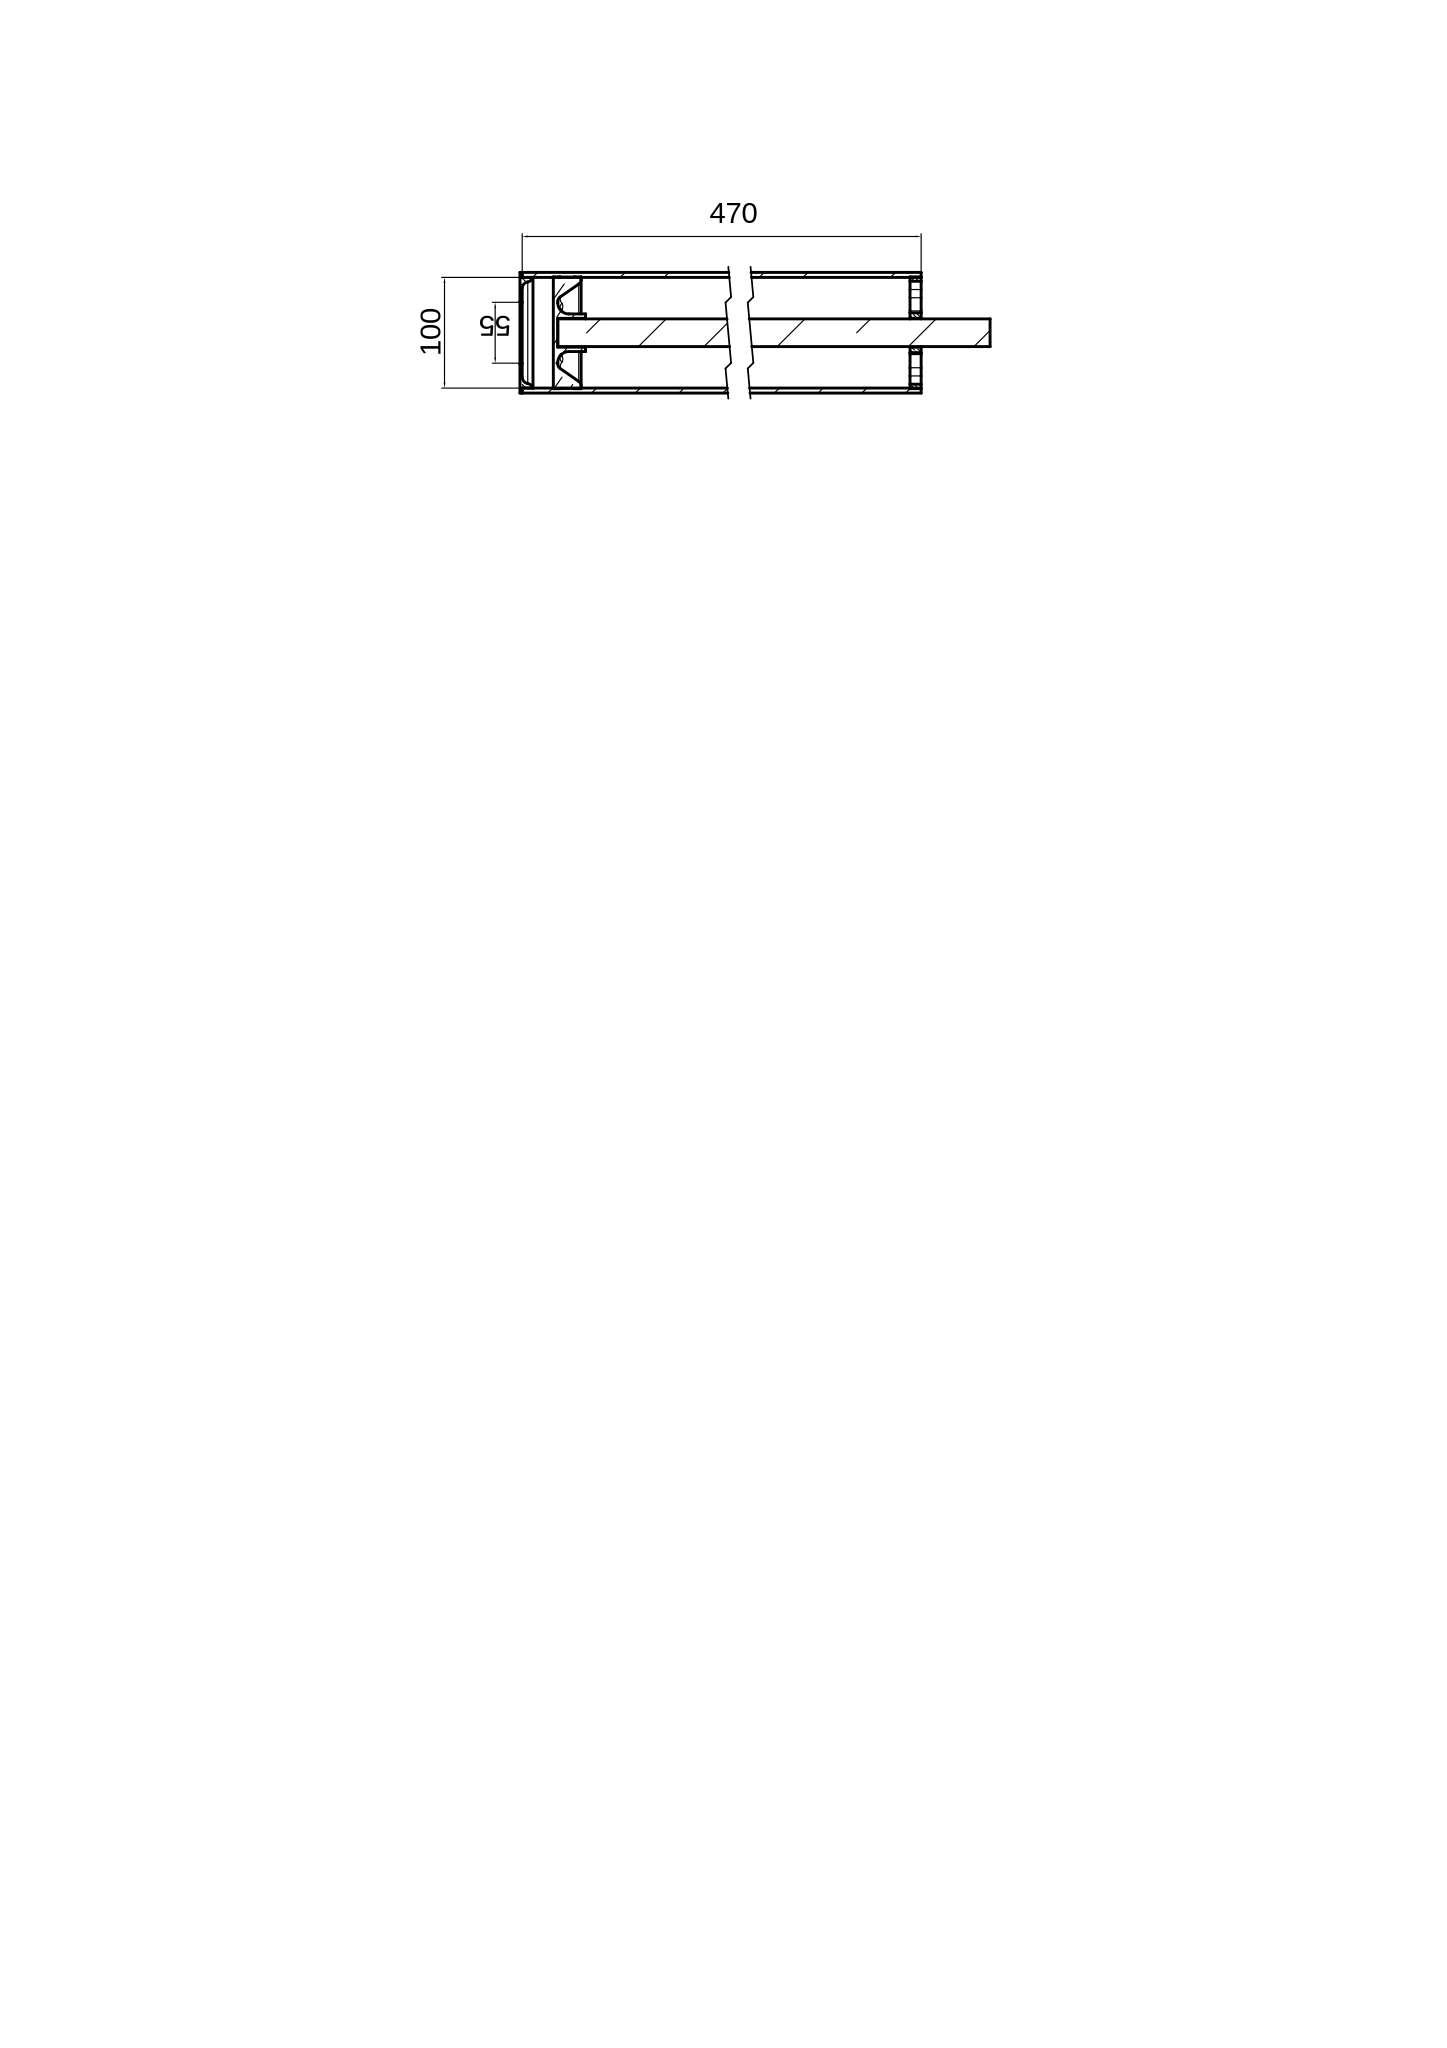
\includegraphics[width=0.8\textwidth]{papers/wirbelringe/fig/zeichnung.pdf}
\caption{Zeichnung und masse der Wirbelringkanone \cite{Wirbelringe:3D_modelle} \label{buch:papers:Wirbelringe:fig:zeichnung}}
\end{figure}
Für den Bau wird ein (oder Zugang zu einem) 3D-Drucker benötigt, \diameter 100 PVC Abflussrohr und eine Möglichkeit, Rauch zu erzeugen, um die Wirbelringe sichtbar zu machen. 
\index{Rauch}%
Es müssen lediglich alle Teile 3D-gedruckt (siehe \cite{Wirbelringe:3D_modelle}) und anschliessend mit einem PVC-Kleber fixiert werden. 
Die Konstruktion ist in Abbildung \ref{Wirbelringe:fig:zeichnung} dargestellt.

\subsection{Versuche}

\subsubsection{Wirbelringe erzeugen\label{Wirbelringe:wirbelringeerzeugen}}

Um nun mit dieser Wirbelringkanone Wirbelringe zu erzeugen, muss der Kolben vollständig zurückgezogen werden und die entstehende Kavität mit möglichst dichtem Rauch oder Nebel gefüllt werden.
\index{Wirbelringkanone}%
Für langanhaltende Wirbelringe sollte ein möglichst windstiller Durchführungsort gewählt werden.
Zum Erzeugen von Wirbelringen muss lediglich der Kolben nach vorne bewegt werden.
Aus Gleichung \eqref{Wirbelringe:eq:naeherungZirkulation} ist ersichtlich, dass sowohl die Länge als auch die Geschwindigkeit, die der Kolben bewegt wird, relevant ist.
Daher brauch es eventuell mehrere Versuche, damit ein Wirbelring entsteht.
Kurze, ruckartige Bewegungen sind dabei langen, langsamen Bewegungen vorzuziehen.

\subsubsection{Wirbelringe teilen}
\index{Wirbelring teilen}%
Aus Abschnitt \ref{Wirbelringe:Grenzflaechen} ist bekannt, dass Wirbel nur auf Grenzflächen oder sich selbst enden können. 
Um das bei einem Wirbelring aufzuzeigen, kann ein Wirbelring ``gespalten'' werden. 
Ein Wirbelring soll dazu gebracht werden, die Grenzflächen von sich selbst auf etwas anderes, zum Beispiel ein Tisch, zu ändern. 
Mithilfe einer Kante, die wie eine Klinge funktioniert, kann der Wirbelring geschnitten und so umgelenkt werden, dass der jetzige Wirbelfaden sich weiter bewegt. 
Dieser Versuch ist in Abbildung \ref{Wirbelringe:fig:wirbelringversuch} dargestellt und beinhaltet folgenden Ablauf:

\begin{figure}
    \centering
    \subfigure[\label{Wirbelringe:fig:versuch_moment_1}]{
        %\includegraphics[width=0.3\textwidth]{papers/wirbelringe/fig/versuch_moment_1.png}
        \includegraphics[width=0.3\textwidth]{papers/wirbelringe/fig/versuch_moment_1.jpg}
    }\hfill
    \subfigure[\label{Wirbelringe:fig:versuch_moment_2}]{
        %\includegraphics[width=0.3\textwidth]{papers/wirbelringe/fig/versuch_moment_2.png}
        \includegraphics[width=0.3\textwidth]{papers/wirbelringe/fig/versuch_moment_2.jpg}
    }\hfill
    \subfigure[\label{Wirbelringe:fig:versuch_moment_3}]{
        %\includegraphics[width=0.3\textwidth]{papers/wirbelringe/fig/versuch_moment_3.png}
        \includegraphics[width=0.3\textwidth]{papers/wirbelringe/fig/versuch_moment_3.jpg}
    }
    \caption{3D Darstellung in Blender des gewünschten Versuchsausgangs.}
    \label{Wirbelringe:fig:wirbelringversuch}
\end{figure}


\begin{enumerate}
    \item Abbildung \ref{Wirbelringe:fig:versuch_moment_1}: Ein Wirbelring wird auf eine Kante gerichtet erzeugt.
    \item Abbildung \ref{Wirbelringe:fig:versuch_moment_2}: Dieser Wirbelring trifft auf die Kante und übernimmt diese als neue Grenzflächen, da diese etwa parallel zu den vorherigen waren.
    \item Abbildung \ref{Wirbelringe:fig:versuch_moment_3}: Durch leichte Änderungen können sich die Grenzflächen aus der vertikalen in die horizontale Ebene ändern.
    Somit können diese auf eine andere Fläche übergehen.
    Der Wirbelring kann sich so weiter fortbewegen.
\end{enumerate}
    


\printbibliography[heading=subbibliography]
\end{refsection}
